% This is samplepaper.tex, a sample chapter demonstrating the
% LLNCS macro package for Springer Computer Science proceedings;
% Version 2.20 of 2017/10/04
%
\documentclass[runningheads]{llncs}
%
\usepackage{graphicx}
\usepackage{amsmath}
\usepackage{algorithm} %format of the algorithm 
\usepackage{algorithmic} %format of the algorithm 
\usepackage{multirow} %multirow for format of table 
\usepackage{amsmath}
\usepackage{xcolor}
\renewcommand{\algorithmicrequire}{\textbf{Input:}} 
\renewcommand{\algorithmicensure}{\textbf{Output:}}

% Used for displaying a sample figure. If possible, figure files should
% be included in EPS format.
%
% If you use the hyperref package, please uncomment the following line
% to display URLs in blue roman font according to Springer's eBook style:
% \renewcommand\UrlFont{\color{blue}\rmfamily}

\begin{document}
%
\title{Contribution Title}
%
%\titlerunning{Abbreviated paper title}
% If the paper title is too long for the running head, you can set
% an abbreviated paper title here
%
\author{Shen Zhengfei\inst{1}\orcidID{0000-1111-2222-3333} \and
Cao Jian\inst{2}\orcidID{1111-2222-3333-4444} }
%
\authorrunning{F. Author et al.}
% First names are abbreviated in the running head.
% If there are more than two authors, 'et al.' is used.
%
\institute{Princeton University, Princeton NJ 08544, USA \and
Springer Heidelberg, Tiergartenstr. 17, 69121 Heidelberg, Germany
\email{lncs@springer.com}\\
\url{http://www.springer.com/gp/computer-science/lncs} \and
ABC Institute, Rupert-Karls-University Heidelberg, Heidelberg, Germany\\
\email{\{abc,lncs\}@uni-heidelberg.de}}
%
\maketitle              % typeset the header of the contribution
%
\begin{abstract}
The abstract should briefly summarize the contents of the paper in
150--250 words.

\keywords{First keyword  \and Second keyword \and Another keyword.}
\end{abstract}
%
%
%
\section{Introduction}
% \subsection{A Subsection Sample}
Classification is the problem of identifying to which a set if categories or sub-populations a new observation belongs, on the basis of a training set of data containing observations or instance whose category membership is known. In many domain, especially for big data and image recognition, classification has become a most hot and significant topic of research~\cite{ref_article1}.In a training set, the information and features of a datum can be formally and numerically represented as a vector (x1,x2,...,xn). In such a n-dimensional features space, the main goal of classification is to estimate the label of a new unlabeled vector from a testing dataset through calculating the similarity among the labeled and unlabeled vectors. Generally, there is a common hypothesis that the training dataset and the testing dataset has a semblable distribution. 

As a well known and widely used method, the k nearest neighbor (KNN) method, looked on as the most simple but effective method among many available classification method such as bayesian method, support vector machine and neural network. Due to its simplicity but good performance, the kNN algorithm has been considered as a top-10 data-mining method~\cite{ref_article2}. Known as a supervised learning algorithm, its working mechanism is fairly easy to grasp: for a given test sample, KNN algorithm try to get the nearest k samples in the training data set based on a specific distance metric, and then predict according to the information of these samples. In a classification problem, the vote method is usually applied to predict the class of one test samples. i.e. label this sample the most common class among the k nearest neighbors. In the past few decades, some researches are also carried on to replace the vote method with other case based reasoning method, for instance, ~\cite{ref_article3}~\cite{ref_article4} used evidence KNN based on the Dempster-Shafer Theory to extend the classical vote method.

Also, there are two issues often come into being discussed in the research: The First is about the similarity and distance compute between different vectors. recently many new algorithm has been proposed to solve this issue, Lin et al. ~\cite{ref_article5} proposed a similarity compute method via fusing neighborhood information. In this proposed algorithm, both the euclidean distance and the neighbor information is considered simultaneously, the two metric is combined together to measure the similarity between samples. Yung-Kyun Noh et al.~\cite{ref_article6} proposed a generative metric learning method to enhance the performance of kNN algorithm. The second issue is about the selection of optimal value of k for a given data set. The general kNN algorithm simply  assume the whole data set share a same value of k, which is actually not proper and inaccurate for a finite and non-uniformly distributed data set.Recently, many new method has been generate to find the k value adaptively or determine a k value for different sample respectively,  Nicolás García-Pedrajas et al. ~\cite{ref_article7} propose a algorithm to obtain local k value with a simple and fast procdeure, Zhang et al. ~\cite{ref_article8} propose to learn a correlation matrix to reconstruct test data points by training data to assign different k values to different test data points.

The drawbacks of the foregoing methods is obvious, they ignore the uncertainty the training data sample itself. As we all know, the training dataset is composed of a group of labeled data samples, the label itself usually decided by some experts however, could be imprecise or even incorrect.While the label information of the k neighbors is combined to make the ultimate decision, the uncertainty of each point also accumulate. In this case, the accuracy of the kNN algorithm will decrease to some extent. Fortunately, a lot of additional and available information can used to quantify the uncertainty of the label of the sample itself. In a recommendation system, a rate of users or votes of experts of a history result could be considerated when quantify the uncertainties. For instance, Zhu et al.~\cite{ref_article9} described a a real-world decision support system for multi-disciplinary treatment called MdtDSS, the core recommend system predict a new patient's therapeutic regimen based on the historic patients. The ultimate therapy of one patient is voted by a group of doctor which reflect the doctors' opinion. The vote result of one doctor express if he/she approve the ultimate therapy of this person. Obviously, we can construct some connection between the vote result and the uncertainties.

In this paper, we define a method to quantify the uncertainties of samples in the training dataset with extra information, later, we fuse both the uncertainty and the label information as the evidence of that sample in the k nearest neighbors. Then, as to combine all these evidences, we use Dempster-shafer theory to accumulate  all these evidences to decide which class a test sample belongs to. Later, we proposed two strategy to select the optimal k value for a specific test sample based on the combined evidences. At last, we carry on a series of experiments with the data in the MdtDSS mentioned in ~\cite{ref_article9} to verify our method.

This paper is organized as follows: In section 2, we discuss related work on kNN algorithms. In section 3, we introduce the Dempster-shafer evidence theory and the MdtDSS. In section 4, we present the modified evidence-theory based on the uncertainty of data sample and the 2 algorithms upon optimal k value selection for this sample. Finally, in the section 5, we carry on several experiments and present results.


\section{Related Work}
Although the majority vote rule make the kNN algorithm more simple and easier to carry, it is based on a assumption that each of the K nearest neighbors is equally important. In practice, the circumstances can be more complex.Intuitively, the closer the neighbor, the more possible that the unknown vector f will be in the class of this neighbor. In 1995, Thierry Denœux~\cite{ref_article3} unprecedentedly define the frame of discernment ~\cite{ref_article10} of a kNN method, and used  the distance of samples to measure the mass function of one sample. Our own work is a extend to his work.

To replace the majority vote rule, some researchers are also prone to looking on the relationship between the global  and local probability distribution. For a small training data, Sunsern Cheamanunkul ~\cite{ref_article11} propose a simple k-NN rule that takes into account the labels of all of the neighbors, rather than just the most common label. In his approach, relative entropy is used to measure the relationship between the global  and local probability distribution.

\section{Preliminary}
\subsection{Dempster-Shafer theory}
As a generalization of the Bayesian theory of subjective probability, Dempster Shafer theory was proposed in 1976 in ~\cite{ref_article10}. It is a general framework for reasoning with uncertainty data. This theory provide a model to express know and unknown directly of different sources, and the ability to combine all the evidence. It mainly contains 2 crucial steps: Basic Belief Assignment(BBA) and evidence combination.

In the first step, let U represent a non-empty set of mutually exclusive and exhaustive propositions called the frame of decrement. The power set $2^{U}$ is all subsets of the set U, which includes both the empty set  and the entire set U. For the frame of discernment U, the function m:$2^{u}$ $\rightarrow$ [0,1] is a basic probability assignment (BPA) also called a mass function. This function satisfies the following two conditions: 

\begin{equation}
\begin{split}
&(1)\ m(\phi) = 0\\&(2)\ \sum_{A\subset U}m(A) = 1
\end{split}
\end{equation}

m(A) indicates the degree of trust exactly in A. The subsets A of U where m(A) > 0 are called the focal elements of the belief function, and their union is called its core. The function Bel:$2^{u}$ $\rightarrow$ [0,1] is the belief function over U, is defined as the sum of all the masses of subsets:

\begin{equation}
Bel(A) = \sum_{B\subset A}m(B)
\end{equation}

Belief (usually denoted Bel) measures the strength of the evidence in favor of a proposition but not any of its subsets. It ranges from 0 (indicating no evidence) to 1 (denoting certainty). An important difference with probability theory is the sum of belief of a proposition and its negation not necessarily equal to 1. Hence, the remaining belief of A, called total ignorance, is the belief of the whole frame of discernment.

In the second step, Dempster Shafer define a method to combine two or more mass assignments of a same frame of discernment in specific situations. To combine there assignments means to accumulate all evidence from all sources in one frame.This rule derives common shared beliefs among multiple sources and ignores all the conflicting (non-shared) beliefs through a normalization factor. 

Given n mass functions $m_1$,$m_2$...$m_n$ on the same frame of discernment U, for arbitrary A  included in U, the combination rule is as follow:


\begin{equation}
\begin{split}
&\ m_{1,2,...,n}(\phi) = 0\\
&\ 
\begin{split}
m_{1,2,...,n}(A)  &\ =(m_1\oplus m_2 \oplus \cdots 
\oplus m_n)(A) \\
&\ = \frac{1}{K} \sum_{A_1 \cap A_2 \cap \cdots
\cap A_n} m_1(A_1) \cdot m_2(A_2) \cdots m_n(A_n)
\end{split}
\end{split}
\end{equation}

where:

\begin{equation}
\begin{split}
K &\ = \sum_{A_1 \cap A_2 \cap \cdots
\cap A_n \ne \phi} m_1(A_1) \cdot m_2(A_2) \cdots m_n(A_n) \\
&\ = 1 - \sum_{A_1 \cap A_2 \cap \cdots
\cap A_n = \phi} m_1(A_1) \cdot m_2(A_2) \cdots m_n(A_n) 
\end{split}
\end{equation}

the K called Normalization factor is a measure of the amount of conflict among mass functions. 

\subsection{Dempster-Shafer theory based kNN algorithm}

Also known as the evidence-theory based kNN (EKNN) ,the Dempster-Shafer theory based kNN algorithm was proposed by Thierry Denux ~\cite{ref_article3} in 1995. He first established the connection between the multidimensional vector space in the KNN algorithm and the frame of discernment in DS evidence theory. In this approach, each neighbor of a pattern is considered as evidence supporting some hypotheses about the class membership of that pattern. The BPAs are calculated for each of the k nearest neighbors. The belief of each hypothese is obtained by aggregating BPAs using Dempster’s rule of combination. His contribution can be summarized as 2 points: (1)generalized a way to compute the BPA value of  the each k nearest neighbor respectively based on the distance to the unlabeled data sample (2) applied the combination rule into the kNN algorithm with a special form. Our own research take both the DS evidence theory and the uncertainty of neighbors is a extension to Thierry's work which will be presented in this section.

In a classification problem, the training data set can be regarded as a collection on N P-dimensional training samples represented by $X=\{x^i=(x_1^i,...,x_p^i)|i=1,...,N\}$  , every sample in the data set belongs to one and only one class from M classes $C=\{C_1,...,C_M\}$. In the very beginning, each sample in the training data is labeled a class in C with a certain degree of uncertainty, which will be discussed in detail in the following section.The labeled data set can be represented as a dualistic relationship (X,L), where L is the set of labels, that can be used to classify new patterns.

In the Dempster-Shafer theory based kNN algorithm, all possible classes set C make up the frame of discernment, to predict the true label of a unlabeled pattern xs equals to assign it to one class in C.

For this unlabeled new pattern $x^s$, the k neighbors based on a specific distance measurement make up a set $\Phi^s$. Each neighbor in $\Phi^s$ provide a piece of evidence whether xs belongs to a specific class Cq in C, the negation of this piece of evidence is totally innocent, i.e. it doesn't refer to  C itself rather than any subsets of C. If we use mass function to represent this piece of evidence, we get the following relationship:

\begin{equation}
\begin{split}
&\ m^{s,i}( \{C_q\}) = \alpha_q
\\
&\ m^{s,i}(C) = 1-\alpha_q
\end{split}
\end{equation}

where i=1,2,...,k.

\begin{definition}
 $\alpha _q$ reflects how much the intensity is that the neighbor $x_i$ support that the unlabeled pattern $x^s$ should be classified as $C_q$.
\end{definition}

According definition 1, the $\alpha _q$ should be a function of distance from xi to $x_s$, because the smaller the distance between  $x_i$ and $x_s$ is,  the more crucial it is to decide wether the class of $x_s$ is the same with the class of $x_i$. Moreover, as the distance between $x_s$ and $x_i$ gets infinitely large, the belief function given by $m^{s,i}$ becomes vacuous, which means that one’s belief concerning the class of $x_s$ is no longer affected by one’s knowledge of the class of $x_i$.

we can replace $\alpha _q$ with any reasonable decreasing function t, here we use the following one:

\begin{equation}
\alpha_q (d^{s,i})= \alpha_0 e^{- d^{s,i} {\beta}}
\end{equation}

Then we can get all the k mass functions of the k nearest neighbors respectively now that the distance to $x_s$ is available. To make the ultimate decision which class $x_s$ belongs to, we should first combine all these pieces of evidence together based on the DS evidence combination rule, according to equation (3), for each class q, we get:

\begin{equation}
\begin{split}
&\ m^{s} _q( \{C_q\}) = 1- \prod_{x^i\in \Phi^s _q } (1-\alpha_q(d^{s,i}))
\\
&\ m^{s} _q(C) = \prod_{x^i\in \Phi^s _q } (1-\alpha_q(d^{s,i}))
\end{split}
\end{equation}

Notice that here the BPA function $m^s_q (\{ C_q \})$ measures the combining belief according to all the neighbors whose class is $C_q$.

Combining all the BPAs $m^s_q$ for each class, a global BPA $m^s=\oplus ^M _{q=1} m^s_q$ is obtained as:

\begin{equation}
\begin{split}
&\ m^{s} ( \{C_q\}) = \frac{m^{s}_q ( \{C_q\})
\prod_{r\neq q} m^s_r(C)}{K}
\\
&\ m^{s} ( C) = \frac{
\prod_{q=1} ^M m^s_q(C)}{K}
\end{split}
\end{equation}

where K is the normalizing factor q=1,2,..,M.

In the last step of the evidence rule based kNN algorithm, for each $C_q$ in C we compute its BPA according to equation (8), and then assign $x_s$ with the optimal class. 

\section{uncertainty and evidence theory based kNN algorithm (UCEkNN)}

In this section, we present our own kNN algorithm based on uncertainty and evidence theory(UCEkNN), and then we proposed 2 optimal k value selection algorithm based on the UCEkNN.

\subsection{UCEkNN}
According to equation (5), till now we use $\alpha _q$ to represent the BPA of one neighbor $x^i$ among k nearest neighbors set  whose class is $C_q$. In practice, however, there is some uncertainty of the label itself. While the BPA of each neighbor is combined, the uncertainties are also accumulated, and the accuracy of the ultimate prediction will decrease to some extent. From this protective, the uncertainty of the label can not be ignored. we define the uncertainty as UC:

\begin{definition}
 $UC^i$ whose value ranges from 0 to 1 describes the uncertainty of the label itself of the neighbor $x^i$ among the k nearest neighbors of $x^s$. $UC^i$ is depended and only depended by the neighbor's characteristic.
\end{definition}

According to definition 2 and equation 5, we proposed a new form for  the BPA function:

\begin{equation}
\begin{split}
&\ m^{s,i}( \{C_q\}) = \alpha_q \cdot {UC}^i
\\
&\ m^{s,i}(C) = 1-\alpha_q \cdot {UC}^i
\end{split}
\end{equation}

Similarly, according to DS combination rule, for each class q:

\begin{equation}
\begin{split}
&\ m^{s} _q( \{C_q\}) = 1- \prod_{x^i\in \Phi^s _q } (1-\alpha_q(d^{s,i} )\cdot UC^i)
\\
&\ m^{s} _q(C) = \prod_{x^i\in \Phi^s _q } (1-\alpha_q(d^{s,i} )\cdot UC^i)
\end{split}
\end{equation}

Although $UC^i$ has been discussed in ~\cite{ref_article3} as the imperfect labeling, our own approach is different intrinsically. In our approach, we do not change the basic form of equation (5), i.e. we assume one neighbor only belongs  to one specific class in spite of uncertainty rather than two or more possible classes. Moreover,  we think $UC^i$ is independent with the distance, and can be accessed easily with some extra information of $x^i$. Here we use a opinion set to describe the extra information, we define it as OpS:

\begin{definition}
 $OpS^i$ describes the extra information set of $x^i$, it can be a set of votes information, ratings information, or other reasonable information which illustrate experts' or users' subjective opinions on whether $x^i$ should be labeled with $C_q$.
\end{definition}

In practical applications, for the kNN algorithm, the label of each sample is decided by a group of people, usually by authoritative experts. $OpS^i$ is such a set which contains the opinions. OpS is accessible in many problems. For example, ~\cite{ref_article9} introduce a medical therapy recommendation system based on kNN algorithm, for each patient in the training data set,  the ultimate therapy is voted by at least 5 doctors. The most voted therapy is used to label this patient. Here, the vote results of doctors' make up the OpS of this patient.

Intuitively, the consistency of doctors' opinions reflects the complexity of making decisions. If all doctors vote to the same therapy, the case of that patient is not complex and clear to make a decision, while for a multi-vote-result situation, the case of that patient can be sophisticated and controversial so that the divergence come out. 

We use the information entropy(IE) ~\cite{ref_article12} of $OpS^i$ to quantify its consistency:

\begin{equation}
H(OpS^i) =- \sum_{c \in C} P_{ic} \cdot log (P_{ic})
\end{equation}

where $P_ic$ is the proportion of class c in $OpS^i$.

Moreover, the uncertainty $UC^i$ of the label of xi has some connection with the uncertainty of $OpS^i$. For a high-consistency case where H($OpS^i$) has a small value, the $UC^i$ should be more close to 1 while for a controversial case where H($OpS^i$) has a large value, he $UC^i$ should be more close to 0. From this prospective, we conclude the $UC^i$ is a decreasing function of H($OpS^i$). We suggest to chose the following function:

\begin{equation}
UC^i=UC_0e^{-H(OpS^i)\beta_u}
\end{equation}

For a query instance of unknown category $x^s$, the predicting process is shown in Algorithm 1.


\begin{algorithm} %算法开始 
\caption{Outline of the proposed Algorithm} %算法的题目 
\label{alg1} %算法的标签 
\begin{algorithmic}[1] %此处的[1]控制一下算法中的每句前面都有标号 
\REQUIRE  a training set $T=\{(x_1,y_1),...,(x_n,y_n)\}, x_i \in \Re ^p$,  a reasonable k, a query instance $x^s$, $OpS^i$ for each sample in training set %输入条件(此处的REQUIRE默认关键字为Require,在上面已自定义为Input) 
\ENSURE the optimal label of $x^s$ %输出结果(此处的ENSURE默认关键字为Ensure在上面已自定义为Output) 
% if-then-else 
\STATE get the k  nearest neighbors set $N=\{(x_1,y_1),...,(x_k,y_k)\}, x_i \in \Re ^p$
% for loop 
\FORALL{$x^i$ in T}
\STATE calculate H($OpS^i$) for each $x^i$ using equation (11)
\STATE  calculate BPA for each $x^i$ using equation (9)
\ENDFOR
\FORALL{classification $C_q$ in C}
\STATE  calculate combining BPA ms($\{C_q\}$) of $C_q$
\ENDFOR
\STATE return the optimal label whose BPA ls the largest

\end{algorithmic}
\end{algorithm}











\subsection{optimal k value selection based on UCEkNN}

Traditional k value selection algorithm aim to find the global optimal k for a fixed training data set and testing dataset.Although a good value might be obtained using cross validation (CV), the same value is unlikely to be optimal for the whole space spanned by the training set. In this brief, we devised a new greedy method based on UCEkNN.

For different k ranging in [$k_min$,$k_max$], the neighbors set of $x^s$ is different, so is the BPA of different classification. Consequently, to search a optimal k for a unlabeled sample is tantamount to determine a best opportunity when the BPA of all classifications meet some optimal condition. Here, we give two available conditions: 

\subsubsection{condition 1}
for different k, the largest value of ms($\{C_q\}$) reaches the maximum

\subsubsection{condition 2}
for different k, the difference between the largest and second largest value of ms($\{C_q\}$) reaches the maximum
Detailed execution steps of our approach under condition 1 and condition 2 are illustrated by Algorithm 2 and Algorithm 3 respectively.

\begin{algorithm} %算法开始 
\caption{Outline of the proposed Algorithm} %算法的题目 
\label{alg1} %算法的标签 
\begin{algorithmic}[1] %此处的[1]控制一下算法中的每句前面都有标号 
\REQUIRE  a training set $T=\{(x_1,y_1),...,(x_n,y_n)\}, x_i \in \Re ^p$,  a reasonable k, a query instance $x^s$, $OpS^i$ for each sample in training set %输入条件(此处的REQUIRE默认关键字为Require,在上面已自定义为Input) 
\ENSURE the optimal label of $x^s$ %输出结果(此处的ENSURE默认关键字为Ensure在上面已自定义为Output) 
\FORALL{k in [$k_{min}$,$k_{max}$]}
    \FORALL{classification $x^i$ in T}
    \STATE  calculate H($OpS^i$) for each $x^i$ using equation (11)
    \STATE  calculate BPA for each $x^i$ using equation (9)
    \ENDFOR
    \FORALL{classification $C_q$ in C}
    \STATE calculate combining BPA ms($\{C_q\}$) of $C_q$
    \ENDFOR
    \STATE get $m^s(A)=max\{m^s(\{C_q\}),C_q \in C\}$
\ENDFOR
\STATE return the optimal label whose BPA ls the largest
\end{algorithmic}
\end{algorithm}

\begin{algorithm} %算法开始 
\caption{Outline of the proposed Algorithm} %算法的题目 
\label{alg1} %算法的标签 
\begin{algorithmic}[1] %此处的[1]控制一下算法中的每句前面都有标号 
\REQUIRE  a training set $T=\{(x_1,y_1),...,(x_n,y_n)\}, x_i \in \Re ^p$,  a reasonable k, a query instance $x^s$, $OpS^i$ for each sample in training set %输入条件(此处的REQUIRE默认关键字为Require,在上面已自定义为Input) 
\ENSURE the optimal label of $x^s$ %输出结果(此处的ENSURE默认关键字为Ensure在上面已自定义为Output) 
\FORALL{k in [$k_{min}$,$k_{max}$]}
    \FORALL{classification $x^i$ in T}
    \STATE  calculate H($OpS^i$) for each $x^i$ using equation (11)
    \STATE  calculate BPA for each $x^i$ using equation (9)
    \ENDFOR
    \FORALL{classification $C_q$ in C}
    \STATE calculate combining BPA ms($\{C_q\}$) of $C_q$
    \ENDFOR
    \STATE get $m^s(A)=max\{m^s(\{C_q\}),C_q \in C\}$
    \STATE get $m^s(B)=max\{m^s(\{C_q\}),C_q \in C \ and \ C_q \ne A\}$
\ENDFOR
\STATE return the optimal label whose BPA ls the largest
\end{algorithmic}
\end{algorithm}

\subsection{optimization of UCEkNN using L-Sure algorithm}
Actually, the influence of the opinion about the data sample's label from different  experts or users should not be identical. For instance, in a medical decision, the opinion of an experienced and proficient doctor could be more crucial. From this prospective, just using entropy of OpS to measure the uncertainty is not reasonable any more.

L-Sure algorithm is devised to intensify the opinion from more authoritative people who vote for the label of a sample. The basic idea of L-Sure algorithm can be described as two steps: (1) select L most authoritative experts out of the vote set. (2) calculate the uncertainty based on the opinion of these L experts.
Given an unlabeled sample and its k neighbors, a straightforward strategy to pick the L most reliable experts is just sort all the experts by the precision in the k neighbor from high to low. Such a idea is easy but efficient.

After getting the L experts for an unlabeled sample, the uncertainty can be calculated by the following condition: (1) if all the L experts hold the same opinion, then the UCi in equation (9) equals 1 (2) if one or more experts out of L experts hold different opinions, then we still use eqution (12) to calculate the $UC^i$.

All the above steps can be described as equation (13):

\begin{equation}
UC^i=
\begin{cases}
UC_0& \text{condition 1}\\
UC_0e^{-H(OpS^i)\beta_u}& \text{condition 2}
\end{cases}
\end{equation}

\section{Experiment and Discussion}
\subsection{experiment for UCEkNN and optimal k value selection}
To testify our proposed two models(UCEkNN, optimal k value selection), we conduct two experiments which is \textbf{experiment I} (for UCEkNN) and \textbf{experiment II}(for optimal k value selection) using the same real data set in the MdtDSS mentioned in ~\cite{ref_article9}. The size of the dataset is 3340 if we only used it to examine the general kNN Algorithm, however, only1455 of them contain the voting information which can be used in our uncertainty based method. 

In the 1455 instances which have OpS, the average size of OpS is 8 which means there are 8 doctor voting to one patient on average. We repeat the two experiment 3 times respectively based on 3 different subsets of the 1455 instances. Each of the subsets are divided into 3 segments which have different function. The 3 segments are training data set, verification data set and testing data set. \textbf{experiment I and II} use different part of the 3 segments: (1)\textbf{experiment I} use the training data set (2) \textbf{experiment II} using the training data set, verification data set and testing data set at the same time. The length of each segment during the 3 reduplicative experiments is illustrated as follows:

\begin{table}
\begin{center}
\caption{length of each segment during the 3 reduplicative experiments.}\label{tab1}
\begin{tabular}{|c|c|c|c|}
\hline
experimental number &  training & verification & testing\\
\hline
1 & 1028 & 212 & 215\\
2 & 790 & 238 & 427\\
3 & 610 & 347 & 239\\
\hline
\end{tabular}    
\end{center}
\end{table}

In  \textbf{experiment I}, we predict the label of each instance in the testing data set using two method (1) the usual DS evidence rule based kNN Algorithm, and (2) our proposed uncertainty based kNN algorithm (UCEkNN). In this experiment, we use the globally optimal k as the input of these two algorithms. First of all, we devise a simple greedy algorithm: select k in [$k_{min}$,$k_{max}$]  successively and calculate the predicting accuracy with our proposed UCEkNN, and the optimal k is who has the best accuracy. Whereafter, we compare the forecast result and the actual result to judge if the prediction is correct, at last we calculate the accuracy of this experiment. The results of all these 3 reduplicative experiments are as follows:

\begin{table}
\begin{center}
\caption{results of all these 3 reduplicative experiments}\label{tab1}
\begin{tabular}{|c|c|c|}
\hline
experimental number &  EkNN & UCEkNN\\
\hline
1 & 59.53\% & 66.05\%\\
2 & 63.00\% & 66.04\% \\
3 & 58.16\% & 64.01\%\\
\hline
\end{tabular}    
\end{center}
\end{table}

In \textbf{experiment II}, we want to exhibit the improvement we made compared to a fixed globally optimal k if we use different k acquired by our proposed method. Thus, we use (1) the fixed globally optimal k (2) different k acquired by the Algorithm 2 (3) different k acquired by the Algorithm 3 separately to predict the label of each instance in testing data set based on UCEkNN and compute the accuracy, we get:

\begin{table}
\begin{center}
\caption{results of all these 3 reduplicative experiments}\label{tab1}
\begin{tabular}{|c|c|c|c|}
\hline
experimental number &  fixed k & diff k based on Alg.1 & diff k based on Alg.2\\
\hline
1 & 66.05\% & 70.70\%& 69.30\%\\
2 & 66.04\% & 69.79\%& 69.09\% \\
3 & 64.01\% & 67.36\%& 67.78\%\\
\hline
\end{tabular}    
\end{center}
\end{table}

The \textbf{experiment II} felicitously simulate a realistic scene where the kNN is used to predict a new pattern. In such a scene a unlabeled instance get its label then become a historical instance and turn into a part of the training set. It is inflexible and unadvisable to keep a fixed k nor calculate a new optimal k at a regular interval. In contrast, our proposed method get a good performance in the accuracy and can saving huge computing resources.

\subsection{experiment for optimization based on L-Sure algorithm}
To verify the efficiency of our proposed L-Sure algorithm and intensify the comparison against the normal UCEkNN algorithm, we conduct an experiment using the same data set with experiment 2,    and the capacity of the training, verification, and testing data set is  610,347,239 respectively. In our experiment, the value of L varies in the range of 0 to 16, and the result is as follows:

\begin{figure}
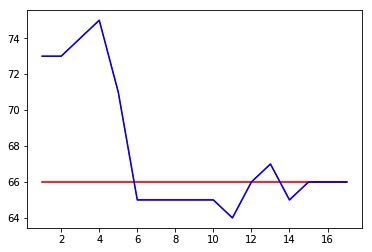
\includegraphics[width=\textwidth]{fig.jpg}}
\caption{the red curve represents the normal UCEkNN while the blue curve represents UCEkNN with L-Sure algorithm. This figure shows that when L meets 6 to 11, the error times is lower than that without using L-Sure algorithm.} \label{fig1}
\end{figure}




\begin{thebibliography}{8}
\bibitem{ref_article1}
Zhu, Xiaofeng , X. Li , and S. Zhang . "Block-Row Sparse Multiview Multilabel Learning for Image Classification." IEEE TRANSACTIONS ON CYBERNETICS 46.2(2016):450.

\bibitem{ref_article2}
Wu, Xindong , et al. "Top 10 algorithms in data mining." Knowledge and Information Systems 14.1(2008):1-37.

\bibitem{ref_article3}
Denoeux, Thierry . "A k-nearest neighbor classification rule based on Dempster-Shafer theory." Systems Man & Cybernetics IEEE Transactions on 25.5(1995):804-813.

\bibitem{ref_article4}
Wang, Lei , L. Khan , and B. Thuraisingham . "An Effective Evidence Theory Based K-Nearest Neighbor (KNN) Classification." 2008 IEEE/WIC/ACM International Conference on Web Intelligence and Intelligent Agent Technology IEEE, 2009.

\bibitem{ref_article5}
Lin, Yaojin , et al. "A new nearest neighbor classifier via fusing neighborhood information." Neurocomputing 143(2014):164-169.

\bibitem{ref_article6}
Noh, Yung Kyun , B. T. Zhang , and D. D. Lee . "Generative Local Metric Learning for Nearest Neighbor Classification." IEEE Trans Pattern Anal Mach Intell PP.99(2018):106-118.

\bibitem{ref_article7}
Garciapedrajas, Nicolas , J. A. R. Del Castillo , and G. Cerruelagarcia . "A Proposal for Local k Values for k-Nearest Neighbor Rule." IEEE Transactions on Neural Networks & Learning Systems 28.2(2015):470.

\bibitem{ref_article8}
Zhang, Shichao , et al. "Learning k for kNN Classification." ACM Transactions on Intelligent Systems and Technology 8.3(2017):1-19. 

\bibitem{ref_article9}
Zhang, Yan , et al. "A Multi-disciplinary Medical Treatment Decision Support System with intelligent treatment recommendation." IEEE International Conference on Computer & Communications IEEE, 2017.

\bibitem{ref_article10}
Rota, Gian Carlo . "297 ppG. Shafer, A Mathematical Theory of Evidence, Princeton University Press (1976). " Ade Bulletin 2(1977):N/A.

\bibitem{ref_article11}
Cheamanunkul, S , and Y. Freund . "Improved kNN Rule for Small Training Sets." International Conference on Machine Learning & Applications IEEE, 2014.

\bibitem{ref_article12}
R Grey. Entropy and Information Theory. ENTROPY AND INFORMATION THEORY. 2012.


\end{thebibliography}
\end{document}
